\section{Example 1 - Infinite Bus}
\label{sec:ex_1}
In this section, we assess how the proposed methods can be applied to study the stability of a converter connected to the infinite bus system described earlier. Moreover, we address the conservativeness limitation showed in Section \ref{sec:lim} and how this can be resolved with a proper choice of the weighting matrix $W_i(s)$.

\subsection{Virtual Admittance compensation}
Figure \ref{fig:GFM_gain_phase_test} shows that, even when both systems are sectorial, the small-phase eigenvalue bounds are highly conservative for frequencies below $50$ Hz. This conservatism arises from the fact that both of $Y_C$ and $Y^{-1}_{net}$ exhibit large phases, and, recalling \eqref{eq:phase_bound}, the small-phase bound is derived under a worst-case assumption, pairing maxima with maxima and minima with minima. However, favorable phase interactions may occur in the product $Y_CY^{-1}_{net}$, leading to partial compensation and a reduction of its eigenvalues' phase. This phenomenon is evident in Figure~\ref{fig:phase-bounds_Yv}, where the small-phase bounds $\Phi(Y_C)+\Phi(Y_{net}^{-1})$ clearly overestimate the actual eigenvalues' phase $\angle\lambda(Y_CY_{net}^{-1})$.
\begin{figure}
    \centering
    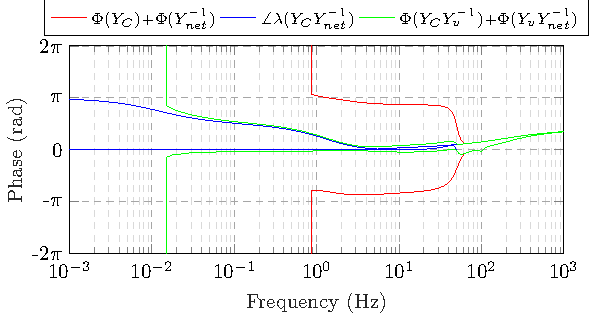
\includegraphics[width=\linewidth]{Phase_Bounds.pdf}
    \caption{Small-phase bounds without and with virtual admittance compensation.}
    \label{fig:phase-bounds_Yv}
\end{figure}

A tighter bound can be obtained by reducing the large phase spread of the numerical range, and therefore limiting the extreme combinations of phases. Since the converter implements a virtual admittance control $Y_v(s)$, and its behavior around $50$ Hz is mainly determined by the virtual admittance, we can post-multiply $Y_C(s)$ by the inverse of $Y_{v}(s)$, such that $Y_{C}(s)Y_{v}(s)^{-1}\approx I$ around those frequencies. The network admittance is transformed accordingly to $Y_{net}(s)Y_{v}(s)^{-1}$.
%we select the post-multiplication matrix $\mathcal{F}(s)=Y_{virt}(s)^{-1}$ (with $\mathcal{E}=I$, $\mathcal{C}=0$). So that we obtain $\tilde{J}_c(s)\approx I$. Meanwhile, $\tilde{J}_{net}(s)= Y_{net}(s)Y_{virt}(s)^{-1}$. 
From another viewpoint, a known dynamic behaviour is shifted from the converter to the network, thereby avoiding the conservatism. In~\eqref{eq:freq_dep_tf_better}, this correspond in the the selection $W_i(s)=Y_v(s)^{-1}$.

Figure~\ref{fig:phase-bounds_Yv} illustrates the effect of this compensation. It can be seen that applying the proposed virtual admittance filtering leads to noticeably improved bounds.
%This figure also highlights the necessity of the translation term $\mathcal{C}$. Since one eigenvalue’s phase approaches $\pi$ at low frequencies and pre-/post-multiplication does not alter it, we must rely on the small gain at those frequencies to ensure stability. Conversely, with a properly chosen $\mathcal{C}$, the stability assessment can rely solely on the phase criterion, as discussed in the next subsection.

At first glance, this approach may appear to undermine the decentralized nature of the certificate. However, in practice, exact knowledge of the virtual admittance values (that is, the behavior around $50$Hz) is not required, and approximate values are sufficient, as shown afterwards. In a decentralized setting, these values can either be selected apriori as fixed parameters or assigned differently across units by the stability certifier. In any case, proposed grid codes for grid-forming converters already define fixed ranges for the effective impedance~\cite{entsoe}. 
\begin{rem}
%Notice in Figure \ref{fig:phase-bounds_Yv}, how one eigenvalues tends to $\pi$ for frequency going to zero, and at the same time small-gain does not guarantee it has module less than one, than stability is difficult to assest. Therefore, here it is evident the need of shift introduced by the $\mathcal{C}$, which can place the eigenvalues in better position where bounding it is easier.
%\color{red}
Figure~\ref{fig:phase-bounds_Yv} shows one eigenvalue approaches $\pi$ as the frequency tends to zero. In this region, the small-gain condition does not ensure $|\lambda|<1$, rendering stability assessment inconclusive. This motivates the shift introduced by $\mathcal{C}$, which relocates the eigenvalues of the open-loop transfer function in a more suitable region where small-phase allows to certify stability.% \color{black}
\end{rem}
%In Figure~\ref{fig:phase-vi-filt}, the small-phase criteria is shown when the post-filter $Y_{virt}(s)$ is used. We can notice that, compared to Figure \ref{fig:GFM_gain_phase_test}, the phase spread of each system is reduced and the phase margin between converter and network is increased.

%\begin{figure}[tbh]
%    \centering
%    \includegraphics[width=\linewidth]{Figures/GFM_InfBus_Yvirt/Phase.pdf}
%    \caption{Small phase condition of a GFM converter with virtual admittance post-filtering.}
%    \label{fig:phase-vi-filt}
%\end{figure}
\subsection{Full transformation}
In Figure~\ref{fig:phase-dep-frame}, the small-phase criteria is shown with the frequency-depended transformation \eqref{eq:generic_trasnf}, with matrices defined as in~\eqref{eq:freq_dep_tf_better}. The cut-off frequency of the filters is set to $0.5$ Hz.  Compared to the previous results, we can obtain sectoriality for the full frequency range and the closed-loop system stability is guaranteed by the small-phase conditions alone.
%\color{red}
This means that the stability of this GFM converter does not depend on the grid strength, meant as its gain, and stability is preserved under both weak and strong conditions. In this sense, the small-phase condition provides a grid-strength-independent stability guarantee. However, variations in the network characteristics, such as changes in the $R/X$ ratio or loading, may alter the network phase. Such variations can reduce the phase margin and potentially drive the converter toward instability.
%\color{black}

\begin{figure}
    \centering 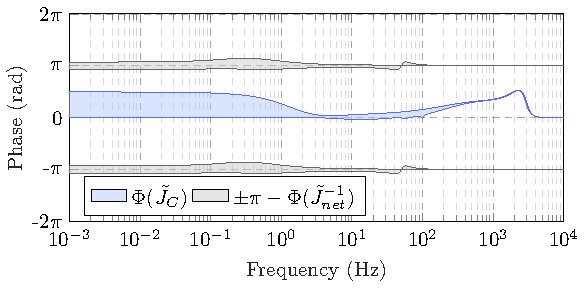
\includegraphics[width=\linewidth]{Phase_mixed.pdf}
    \caption{Small phase condition of a GFM converter with frequency-dependent transformation \eqref{eq:generic_trasnf}, \eqref{eq:freq_dep_tf_better}.}
    \label{fig:phase-dep-frame}
\end{figure}

\subsection{Unstable case}
To further validate the method, we examine the sufficient condition of the theorem: if the closed-loop system is unstable, then the small-phase and the small-gain condition must be simultaneously violated at some frequency. In practice, destabilizing a grid-forming converter is not straightforward. Following \cite{de2012automatic}, we introduce a purely resistive load at the PCC and increase the infinite bus impedance. By switching the control mode to constant-Q and reducing the VSM damping of the GFM from $0.5$ to $0.05$, the closed-loop becomes unstable, exhibiting sustained oscillations at 1.2 Hz. Figure \ref{fig:GFM_Unstable} illustrates the mixed gain/phase test, considering the proposed transformation. 
Enabling the reactive power control reduces the gain at low frequencies, leading to the small-gain condition to be satisfied.
However, while in the stable case ($D=0.5$) the small-phase condition is satisfied, in the unstable case ($D=0.05$), the converter phase increases substantially, and together with the network phase causes the phase condition to be violated, while the gain condition is also not satisfied around the unstable oscillation frequency.
\begin{figure}
    \centering
    \begin{subfigure}{\columnwidth}
        \centering
        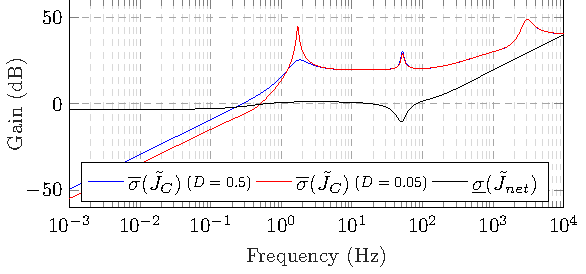
\includegraphics[width=\linewidth]{Gain_inf_un.pdf}
    \end{subfigure}
    \begin{subfigure}{\columnwidth}
        \centering
        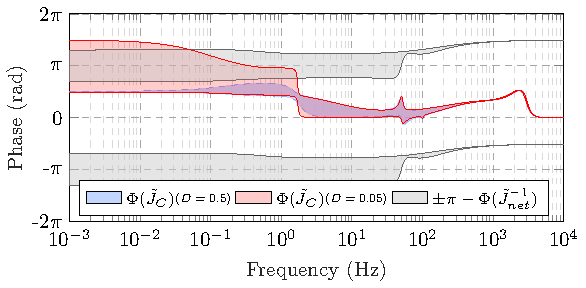
\includegraphics[width=\linewidth]{Phase_inf_un.pdf}
    \end{subfigure}
    \caption{GFM Infinite Bus - Stable ($D=0.5$) vs Unstable ($D=0.05$).}
    \label{fig:GFM_Unstable}
\end{figure}

\section{Example 2 - IEEE 14 Bus System}
\label{sec:ex_2}
\begin{figure}
    \centering
    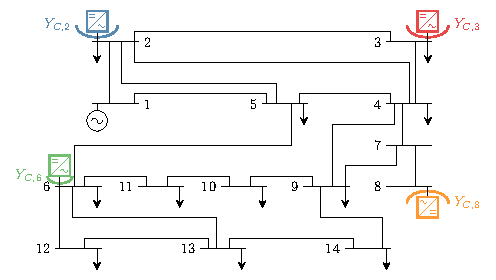
\includegraphics[width=\linewidth]{IEEE14_diagram.pdf}
    \caption{IEEE 14 Bus System diagram}
    \label{fig:ieee14_diagram}
\end{figure}
To extend and show the scalability of our approach, we consider the modified IEEE 14 Bus System shown in Figure \ref{fig:ieee14_diagram}, which parameters are given in \cite{RepoZenodo}. Four GFM converters are connected at the buses 2, 3, 6, and 8.
Similarly to the infinite bus example, to build an unstable case, we select a low damping value for converter 8, connect purely resistive loads, and increase the line 7-8 impedance. In this setup, the system is unstable with an unstable oscillation at 0.54 Hz driven by converter 8.
In Figure \ref{fig:IEEE14_criteria}, the decentralized conditions are shown using the proposed transformation and virtual admittance compensation. While the converters 2, 3, and 6 satisfy the small-phase condition, converter 8 does not. In particular, below 1.64 Hz, its phase overlaps the network phase. This does not imply the instability of the system; however, knowing that the system is unstable, it identifies the responsible converter, and by appropriately retuning its control parameters, stability can potentially be restored. For example, if we apply the same tuning of converter 6, which satisfy the small-phase condition, to converter 8, then stability is recovered.

In this example, each converter implements a different $R/X$ ratio in its virtual admittance, as reported in Table~\ref{tab:virt_adm}, while a fixed value ($R_v=0.01$, $X_v=0.1$) is used for the virtual admittance compensation for all converters. This demonstrates that, even when the exact virtual admittance is unknown, a reasonable estimate can still be used to obtain adequate phase bounds and, consequently, an effective stability validation with the proposed approach.
\begin{figure}
    \centering
    \begin{subfigure}{\columnwidth}
        \centering
        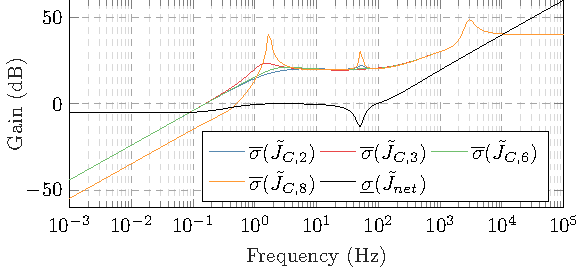
\includegraphics[width=\linewidth]{Gain_14.pdf}
    \end{subfigure}
    %\vspace{-1em} 
    \begin{subfigure}{\columnwidth}
        \centering
        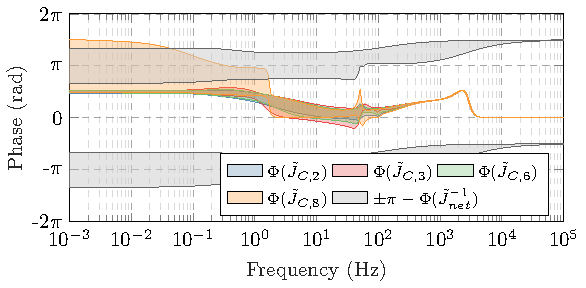
\includegraphics[width=\linewidth]{Phase_14.pdf}
    \end{subfigure}
    \caption{Stability analysis of the 14 Bus System}
    \label{fig:IEEE14_criteria}
\end{figure}

\begin{table}
\centering
\caption{Virtual admittance setting in 14 Bus System}
\label{tab:virt_adm}
\begin{tabular}{ccc}
GFM Bus & $R_v$ (p.u) & $X_v$ (p.u) \\
\hline
$2$ & $0.02$ & $0.1$ \\
$3$ & $0.05$ & $0.1$ \\
$6$ & $0.03$ & $0.1$ \\
$8$ & $0.01$ & $0.1$ \\
\hline
\end{tabular}
\end{table}